% Written by ../code/make_numbers.py. Do not edit by hand.
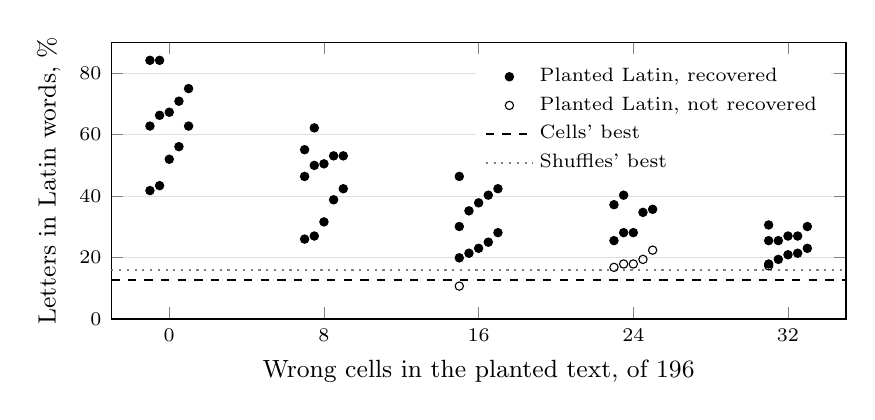
\begin{tikzpicture}
\begin{axis}[width=0.9\linewidth, height=0.42\linewidth,
  xmin=-3, xmax=35, ymin=0, ymax=90, xtick={0,8,16,24,32},
  xlabel={Wrong cells in the planted text, of 196}, ylabel={Letters in Latin words, \%},
  label style={font=\small}, ticklabel style={font=\scriptsize}, ymajorgrids, grid style={gray!25},
  legend style={font=\scriptsize, draw=none, at={(0.98,0.95)}, anchor=north east}, legend cell align=left]
\addplot[only marks, mark=*, mark size=1.5pt, black] coordinates {(-1.0,41.8) (-0.5,43.4) (0.0,52.0) (0.5,56.1) (1.0,62.8) (-1.0,62.8) (-0.5,66.3) (0.0,67.3) (0.5,70.9) (1.0,75.0) (-1.0,84.2) (-0.5,84.2) (7.0,26.0) (7.5,27.0) (8.0,31.6) (8.5,38.8) (9.0,42.4) (7.0,46.4) (7.5,50.0) (8.0,50.5) (8.5,53.1) (9.0,53.1) (7.0,55.1) (7.5,62.2) (15.0,19.9) (15.5,21.4) (16.0,23.0) (16.5,25.0) (17.0,28.1) (15.0,30.1) (15.5,35.2) (16.0,37.8) (16.5,40.3) (17.0,42.4) (15.0,46.4) (23.0,25.5) (23.5,28.1) (24.0,28.1) (24.5,34.7) (25.0,35.7) (23.0,37.2) (23.5,40.3) (31.0,17.9) (31.5,19.4) (32.0,20.9) (32.5,21.4) (33.0,23.0) (31.0,25.5) (31.5,25.5) (32.0,27.0) (32.5,27.0) (33.0,30.1) (31.0,30.6)};
\addlegendentry{Planted Latin, recovered}
\addplot[only marks, mark=o, mark size=1.5pt, black] coordinates {(15.0,10.7) (23.0,16.8) (23.5,17.9) (24.0,17.9) (24.5,19.4) (25.0,22.4) (31.0,17.3)};
\addlegendentry{Planted Latin, not recovered}
\addplot[dashed, thick, black] coordinates {(-3,12.8) (35,12.8)};
\addlegendentry{Cells' best}
\addplot[dotted, thick, gray] coordinates {(-3,16.0) (35,16.0)};
\addlegendentry{Shuffles' best}
\end{axis}
\end{tikzpicture}
